% !TEX root = ../../thesis.tex
%______________________________________________________________________________
%
% SECTION
\section{Results}
\label{section:results}
%
%______________________________________________________________________________

In this section the spectral cell method is applied to a simple problem described in \ref{section:error_calculation} with different discretizations and embeddings, and then to an example with a more complex geometry that has a cell distribution more resembling a practical application. For the simple case, approaches without lumping, with density scaling, and with HRZ lumping are compared.

%______________________________________________________________________________
%
% SUB-SECTION
\subsection{Axis-aligned bar}
\label{section:axis_aligned_bar}
%
%______________________________________________________________________________

A simple straight bar model introduced in \ref{section:error_calculation} is considered. To allow a fictitious domain extension and analyze the behaviour of the SCM, the problem is modeled in 3D instead of one.

\begin{figure}[h]
	\centering
	\includegraphics[height=3.5cm]{figures/bar_axis_aligned}
	\caption{Embedded axis-aligned bar and its discretization.}
	\label{fig:bar_axis_aligned}
\end{figure}

A bar of length $L_x$ with a rectangular cross-section $[L_y \times L_z]$ is symmetrically embedded into a Cartesian domain of size $[L_x \times 2h_y \times L_z]$ that does not conform to the bar in $y$-direction. The domain is discretized by an $[n_x \times 2 \times 1]$ Cartesian grid of identical cells.

The distributed source defined in equation \ref{eq:toy_problem_source} is extended to 3D but only in the physical domain:

\begin{equation} \label{eq:axis_aligned_source}
	f(\mathbf x,t) = \begin{cases}
	e^{-10^4x^2} sin \left( \frac{2 \pi}{T} t \right) & t \in \left[ 0,\frac{T}{2} \right] \land \mathbf x \in \Omega_p \\[0.5em]
	0 & \text{otherwise} \\
	\end{cases}
\end{equation}

\begin{table}[h]
	\centering
	\bgroup
	\def\arraystretch{1.5}
	\begin{tabular}{|c|c|c|c|c|c|c|c|}
		\hline
		\multicolumn{3}{|c}{geometry} & \multicolumn{2}{|c}{material} & \multicolumn{1}{|c}{source} & \multicolumn{2}{|c|}{time} \\
		\hline \hline
		$L_x$ & $h_y$ & $L_z$ & $\rho$ & $E$ & $T$ & $\Delta t$ & $t_{max}$ \\
		\hline
		$0.5$ & $0.01$ & $0.01$ & $1$ & $1$ & $0.1$ & $2\cdot 10^{-4}$ & $0.5$ \\
		\hline
	\end{tabular}
	\egroup
	\caption{Constant parameters for the bar example.}
\end{table}

Time integration is performed using central differences described in \ref{subsection:wave_equation_temporal_discretization} for every case. In the following subsections, the behaviour of solutions obtained by different approaches is studied, depending on various quantities such as the:

\begin{tabular}{>{\textbullet\hspace{\labelsep}}lr}
	number of elements in $x$-direction & $n_x$ \\
	order of basis functions & $p$ \\
	fill ratio of cells & $\eta$ \\
	fictitious exponent & $\beta$
\end{tabular}\bigskip

%______________________________________________________________________________
% SUB-SUB-SECTION
\subsubsection*{Fill ratio}
\label{section:fill_ratio}
%______________________________________________________________________________

Since the mass matrices of uncut cells are inherently diagonal, lumping schemes have no effect on them. However, as the proportion of the physical domain in a cell decreases, the role of lumping becomes more dominant. The fill ratio $\eta$ shows the proportion of the physical domain relative to the total volume of a cell. In the bar example, this is controlled by varying the height $L_y$ of the bar while leaving the mesh untouched to avoid errors originating from element skewness. Hence, the fill ratio can be computed as follows:

\begin{equation} \label{eq:fill_ratio}
	\eta = \cfrac{L_y}{2h_y}
\end{equation}

This value is identical for every cell in the model. To make sure that no errors originate from the adaptive nature of integration, bar's height is always set such that an octree of depth $r$ can perfectly capture its boundary. More precisely, the bar is shrunk sequentially by powers of two: $L_y = 2 ^{-r} \ 2h_y$

\begin{center}
\begin{minipage}[b]{0.45\textwidth}
	\centering
	\bgroup
		\def\arraystretch{2.5}
		\begin{tabular}{|c||c|c|c|c|c|}
			\hline
			$r$ & 0 & 1 & 2 & 3 & 4 \\
			\hline
			$L_y$ & $2h_y$ & $h_y$ & $\cfrac{h_y}{2}$ & $\cfrac{h_y}{4}$ & $\cfrac{h_y}{8}$ \\ 
			\hline
			$\eta$ & $1$ & $\cfrac{1}{2}$ & $\cfrac{1}{4}$ & $\cfrac{1}{8}$ & $\cfrac{1}{16}$ \\
			\hline
		\end{tabular}
	\captionof{table}{Cell fill ratios for different bar heights.}
	\egroup
\end{minipage}
\hfill
\begin{minipage}[b]{0.45\textwidth}
	\centering
	\includegraphics[width=0.75\textwidth]{figures/cell_fill_ratio}
	\captionof{figure}{Example cell for different bar heights.}
\end{minipage}
\end{center}

For all following cases, the number of elements in $x$-direction $n_x=30$ is fixed and p-refinement is performed $p=1,...,4$. The indicator function $\alpha(\mathbf x)$ is characterized by the fictitious exponent $\beta = 5$. Displacements are evaluated at two sample points defined in section \ref{section:error_calculation}, and the relative error defined in equation \ref{eq:time_of_flight_relative_error} is computed using wavelet peaks.

Note, that the mesh conforms to the boundary for $r=0$, which means that no adaptive integration or lumping is performed, and the solution is identical to that of the standard SEM. This case can be used as reference.

Without lumping, the solutions shown in figure \ref{fig:aligned_bar_fill_ratio_no_lumping} converge as expected. Spurious oscillations decay as $p$ increases and the effective wave speed approaches the analytical one. The fill ratio has little impact on the results of embedded setups, but the boundary-conforming case visibly differs from them. This is likely due to the fact that the material in the fictitious domain has non-zero material parameters and introduces errors in the adaptive integration. At higher polynomial orders however, these seem to balance other discretization errors.
Since no lumping is performed, the mass matrix has non-zero off-diagonal entries from the adaptive integration, thus leading to less efficient time integration.

%______________________________________________________________________________
%
% SUB-SECTION
\subsection{Rotated bar}
\label{section:rotated_bar}
%
%______________________________________________________________________________

%______________________________________________________________________________
%
% SUB-SECTION
\subsection{Complex geometry}
\label{section:complex_geometry}
%
%______________________________________________________________________________